%# -*- coding: utf-8-unix -*-
%%==================================================
%% thesis.tex
%%==================================================

% 双面打印
\documentclass[bachelor, openright, twoside]{sjtuthesis}
% \documentclass[bachelor, openany, oneside, submit]{sjtuthesis}
% \documentclass[master, review]{sjtuthesis}
% \documentclass[%
%   bachelor|master|doctor,	% 必选项
%   fontset=fandol|windows|mac|ubuntu|adobe|founder, % 字体选项
%   oneside|twoside,		% 单面打印,双面打印(奇偶页交换页边距,默认)
%   openany|openright, 		% 可以在奇数或者偶数页开新章|只在奇数页开新章(默认)
%   english,			% 启用英文模版
%   review,	 		% 盲审论文,隐去作者姓名、学号、导师姓名、致谢、发表论文和参与的项目
%   submit			% 定稿提交的论文,插入签名扫描版的原创性声明、授权声明 
% ]

% 逐个导入参考文献数据库
% \addbibresource{bib/thesis.bib}
% \addbibresource{bib/chap2.bib}

\begin{document}

%% 无编号内容:中英文论文封面、授权页
%# -*- coding: utf-8-unix -*-
\title{面向海量数据的高效模糊搜索}
\author{刘韵}
\advisor{沈耀}
% \coadvisor{某某教授}
\defenddate{2018年5月31日}
\school{上海交通大学}
\institute{电子信息与电气工程学院}
\studentnumber{5140309455}
\major{计算机科学与技术}

\englishtitle{Efficient approximate search of large-scale data}
\englishauthor{\textsc{Yun Liu}}
\englishadvisor{Prof. \textsc{Yao Shen}}
% \englishcoadvisor{Prof. \textsc{Uom Uom}}
\englishschool{Shanghai Jiao Tong University}
\englishinstitute{\textsc{Depart of Computer Science and Engineering, School of SEIEE} \\
  \textsc{Shanghai Jiao Tong University} \\
  \textsc{Shanghai, P.R.China}}
\englishmajor{Minyi Guo}
\englishdate{May 26th, 2018}


\maketitle

\makeatletter
\ifsjtu@submit\relax
	\includepdf{pdf/original.pdf}
	\cleardoublepage
	\includepdf{pdf/authorization.pdf}
	\cleardoublepage
\else
\ifsjtu@review\relax
% exclude the original claim and authorization
\else
	\makeDeclareOriginal
	\makeDeclareAuthorization
\fi
\fi
\makeatother


\frontmatter 	% 使用罗马数字对前言编号

%% 摘要
\pagestyle{main}
%# -*- coding: utf-8-unix -*-
%%==================================================
%% abstract.tex for SJTU Master Thesis
%%==================================================

\begin{abstract}
	
模糊搜索是一类搜索相同或相似数据的搜索方法。本文针对无感知环境下的大规模人脸数据的模糊搜索,从人脸检测,特征提取与向量匹配三方面进行研究,最终实现了完整的无感知人脸识别系统。

无感知人脸识别系统是一种不依赖待检测者主动配合的人脸识别系统。这种系统利用监控摄像头的实时画面,对其中的人脸进行检测、计数和识别。在教室点名、公司打卡签到等实际场景中有广泛的应用。由于不依赖于被检测人的配合,人脸的图像会呈现偏转、模糊和遮挡等特征,这对检测与识别算法都提出了非常高的要求。

深度学习在人脸检测和特征提取方面有着广泛的应用。本文选取SSH检测器\cite{najibi2017ssh}进行人脸检测,InsightFace\cite{deng2018arcface}进行特征提取。我们还从实际监控摄像中提取数据,建立了无感知人脸检测的测试集CFDDB。并在CFDDB上定义了基准参数,以分析不同人脸检测算法的优劣。

大规模特征向量的匹配是人脸模糊搜索需要解决的另一个问题。本文讨论基于局部敏感哈希与基于有向图的近似搜索算法进行高效的向量匹配,同时给出基于局部敏感哈希匹配算法的优化思路。

无感知人脸识别系统的实现充分考虑了数据处理流程、设备网络拓扑结构、以及系统逻辑架构等的设计,从而使系统具有稳定和可扩展的特性。本文在最后对这部分内容进行了阐述。

\keywords{\large 模糊搜索 \quad 无感知人脸检测 \quad 大规模数据 \quad 向量匹配 \quad 深度学习}
\end{abstract}

\begin{englishabstract}

Approximate search is a type of search method that searches for the same or similar data. This paper focuses on the approximate search of large-scale face data, from the aspects of face detection, feature extraction and vector matching, and finally implements a complete imperceptible face recognition system.

Imperceptible face recognition system is a face recognition system which does not require intentional cooperation from users. This system pulls live images of faces from surveillance cameras at first. Then it performs face detection, face counting and face recognition to get face embeddings. Finally, it matches face embeddings to database contents. This system can be widely used for student attendance management and access control in companies. Since this system does not rely on users’ cooperation, the facial images received would be angled, blurred and occluded, which makes detection and recognition very challenging.

Deep learning has a wide range of applications in face detection and feature extraction. In this paper, we use SSH detector \cite{najibi2017ssh} for face detection and InsightFace\cite{deng2018arcface} for feature extraction. We also pull data from surveillance cameras and present an imperceptible face detection benchmark CFDDB. The benchmark parameters are defined to analyze the performance of different face detection algorithms.

The matching of large-scale feature vectors is another challenge that needs to be solved for approximate search of face data. In this paper, efficient vector matching algorithms based on LSH or directed graph are discussed. At the same time, the optimized method for algorithm based on LSH is given.

We present our system’ s data architecture, physical architecture and logical architecture at the end. This architecture design keeps imperceptible face recognition system efficient, stable and scalable.

\englishkeywords{\large approximate search, imperceptible face detection, large-scale data, vector matching, deep-learning}
\end{englishabstract}



%% 目录、插图目录、表格目录
\tableofcontents
\listoffigures
\addcontentsline{toc}{chapter}{\listfigurename} %将插图目录加入全文目录
\listoftables
\addcontentsline{toc}{chapter}{\listtablename}  %将表格目录加入全文目录
\listofalgorithms
\addcontentsline{toc}{chapter}{\listalgorithmname} %将算法目录加入全文目录

%# -*- coding: utf-8-unix -*-
\begin{nomenclaturename}
\label{chap:symb}

\begin{longtable}{rl}
$recall$     & 召回率 \\
$errorrate$  & 误判率 \\
$\alpha$	 & 检测参数 \\
$\mathbf{q},Q$ & 查询向量 \\
$\mathbf{q}$ & 最邻近向量 \\
$L$			 & Loss函数 \\
$\mathcal{F},\mathcal{G}$ & LSH函数族 \\
$h,g$ 		 & 哈希函数 \\
$d$			 & 距离函数 \\
$\mathcal{M}$& 矩阵空间 


\end{longtable}

\end{nomenclaturename}
 % 主要符号、缩略词对照表

\mainmatter	% 使用阿拉伯数字对正文编号

%% 正文内容
\pagestyle{main}
\include{tex/intro}
\chapter{CFDDB测试集}
\label{chap:establishCFDDB}

在选择正确的算法之前,我们应当选择或者建立一套测试集,以检测算法执行的效果。在人脸检测的领域,已经有数量众多的公开数据集用于训练和测试,常见的有WIDER FACE\cite{yang2016wider},FDDB\cite{fddbTech},LFW\cite{huang2007labeled}等等。然而如图\ref{fig:chap1:pic}所示,这些数据集中的人脸大多是欧美人,而且每张照片中的人脸数量也有限。而我们从监控录像中提取的图片亚洲人偏多,人脸往往是模糊的,大角度的,或是被遮挡的。因此,现有的数据集无法满足我们的测试需求,据此我们建立了自己的数据集CFDDB(Classroom Face Detection Database)。


\begin{figure}[!htp]
	\centering
	\begin{subfigure}{6cm}
		\centering
		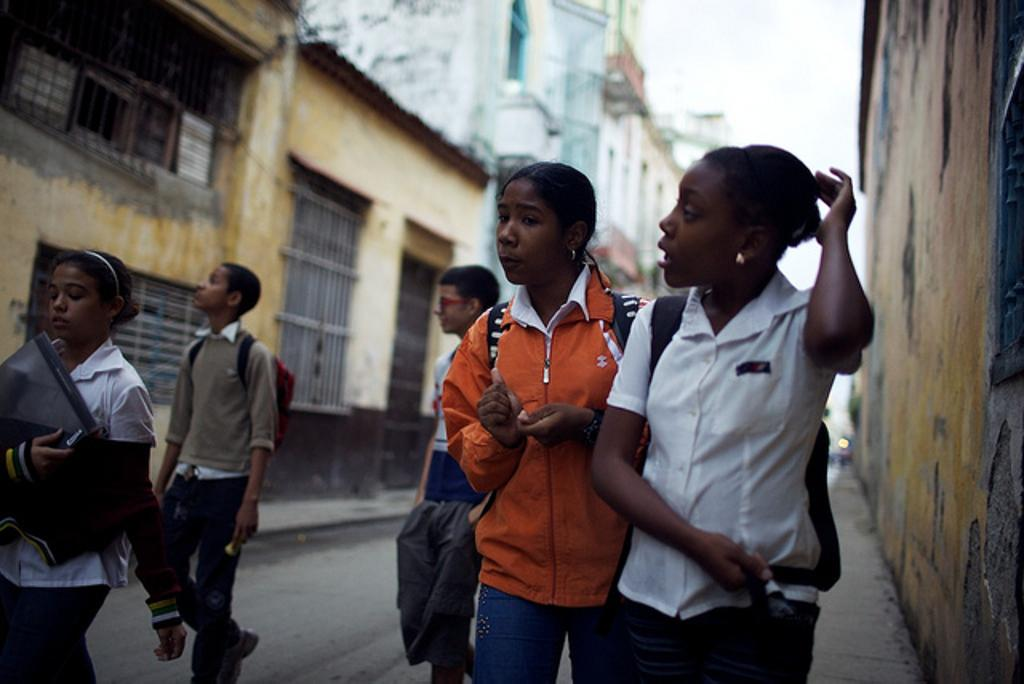
\includegraphics[width=6cm,height=4cm]{chap1/1.jpg}
		\caption{WiderFace 测试集样例图片}
	\end{subfigure}
	\hspace{4em}
	\begin{subfigure}{6cm}
		\centering
		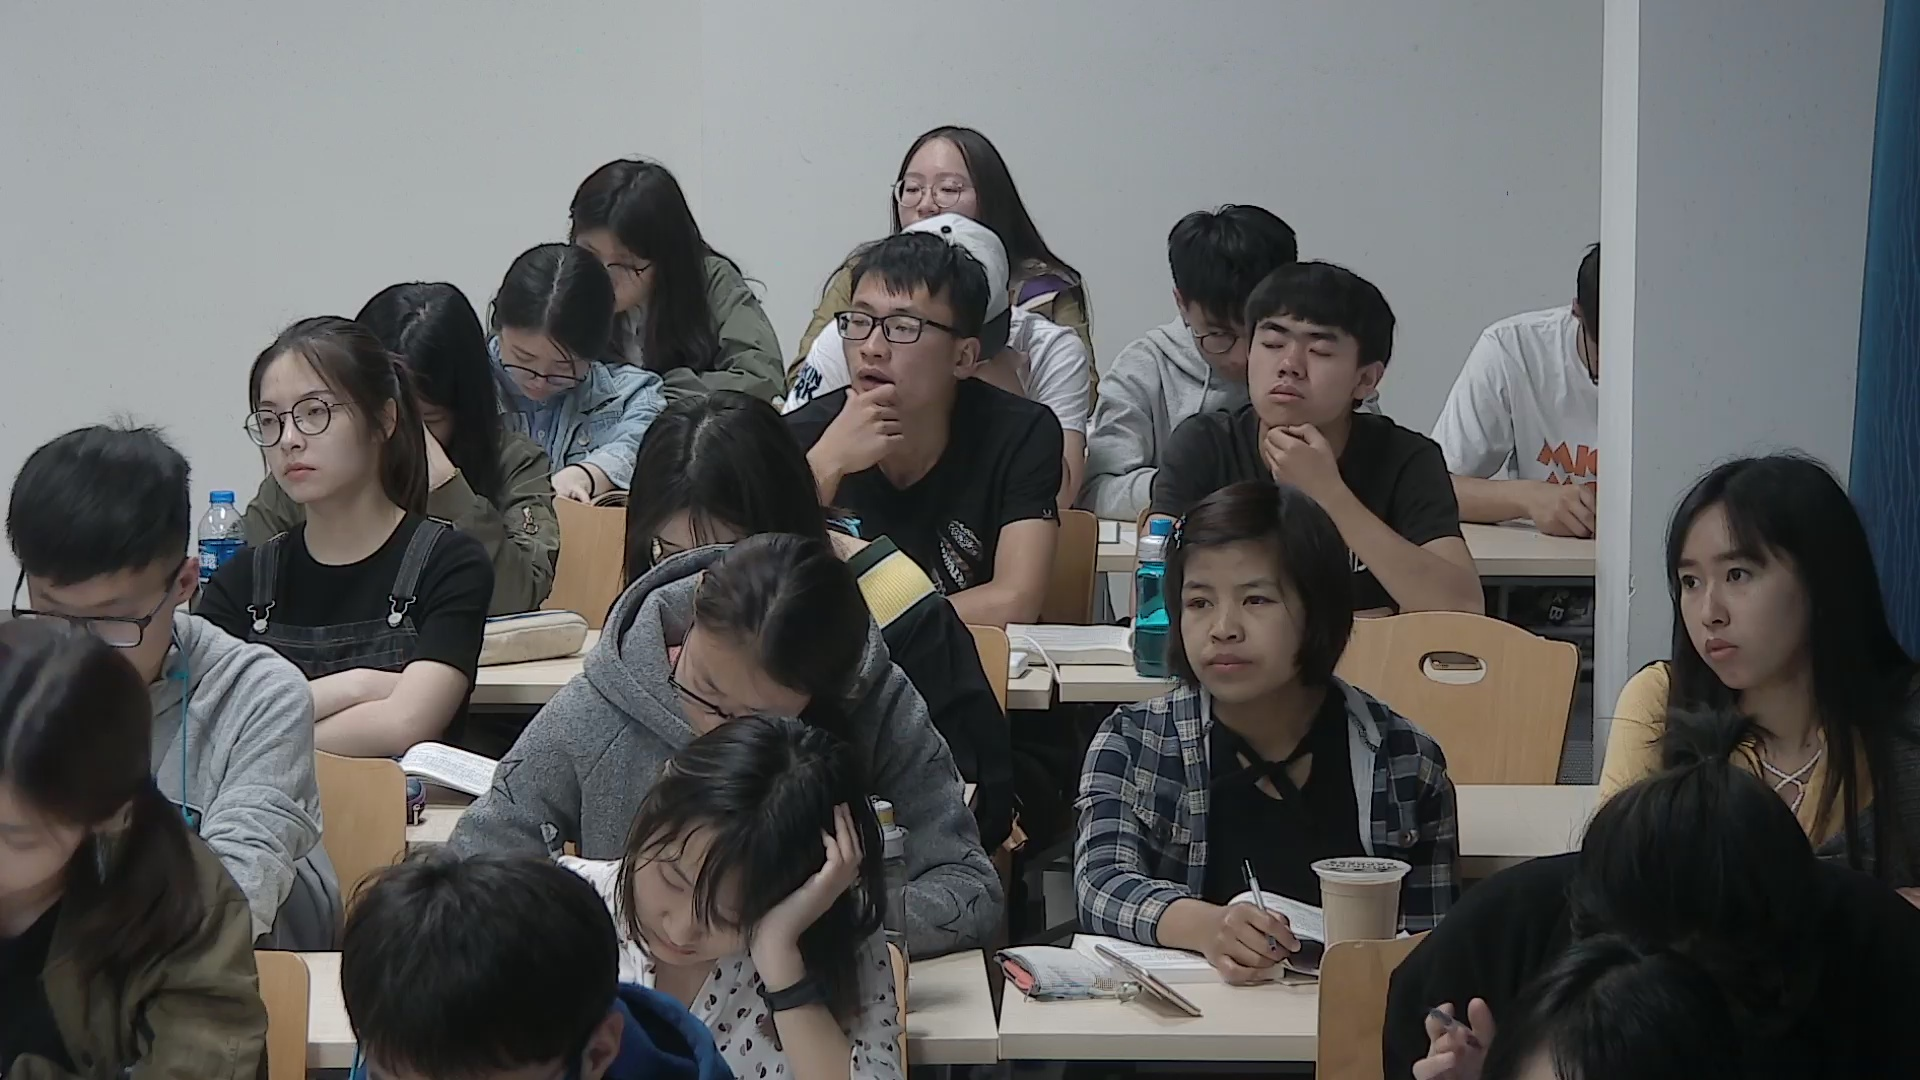
\includegraphics[width=6cm,height=4cm]{chap1/2.jpg}
		\caption{CFDDB 测试集样例图片}
	\end{subfigure}
	\caption{WIDER FACE与CFDDB样例图片对比图}
	\label{fig:chap1:pic}
\end{figure}


\section{CFDDB测试集图片标注规则}

测试集图片由从一段15分钟的监控录像中每隔100帧截取一帧产生,共有149张图片。标注人需要在一张图片中使用矩形框标注全部可识别人脸。标注的矩形框应当以人脸的鼻子为中心,矩形框区域面积应当大概是人脸区域面积的两倍。图\ref{fig:chap1:cfddblbexp}为CFDDB中一张图片的标注可视化之后的效果,其中,绿色的矩形框为标注人标注的人脸区域。

\begin{figure}[!htp]
	\centering
	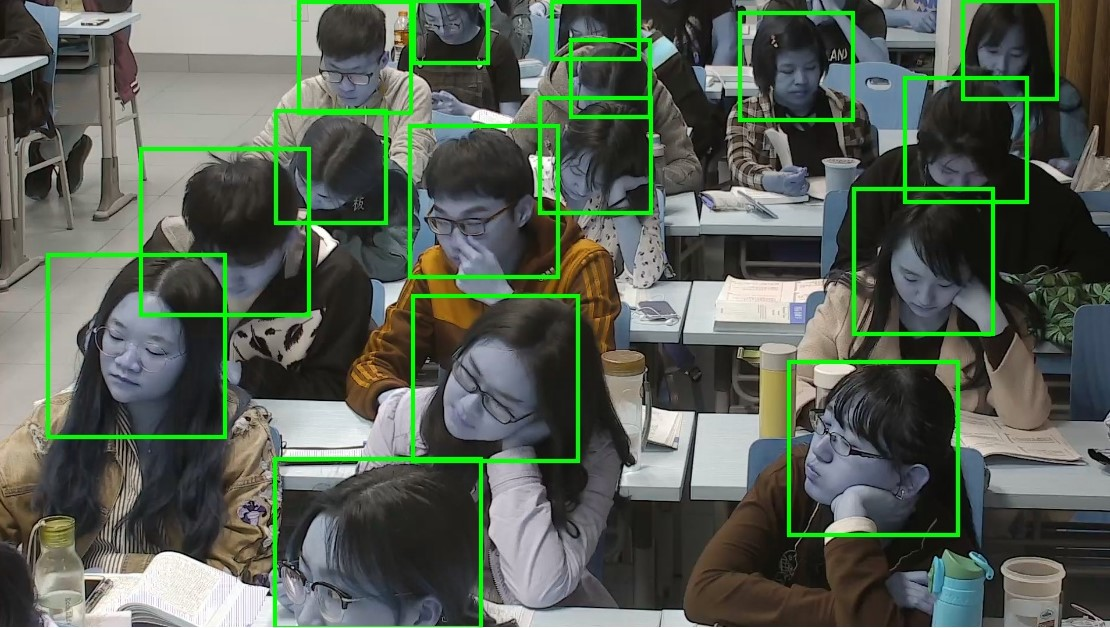
\includegraphics[height=6cm]{chap1/3.jpg}
	\caption{CFDDB 标注示例}
	\label{fig:chap1:cfddblbexp}
\end{figure}

矩形框标注完毕之后需要给每一个矩形框添加一个标签,这个标签是人脸的全局名称。标签添加完毕之后,将一张图片中所有矩形框的位置信息和标签信息写入与图片同名的XML文件进行保存。

为了保证视频中每位老师和同学的隐私,我们给每张人脸添加的全局标签均为一定规则生成的独特的数字组合而不是姓名,以保证数据集不被滥用。

\section{CFDDB测试集的纠错与预处理}

测试集的标注是人为进行的,有可能会出现差错,所以在将标注信息加入测试集之前,还需要对标注的信息进行认真反复的比对,以确保标注信息的正确性。在本次比对中,共发现六处错误。修改所有错误之后,测试集中共有可用图片134张,人脸1087个,总人数84人。

测试集的预处理分为四步。第一步是将所有人脸图像区域切割出来,并将相同的人脸放到以该人脸的标签为名的文件夹下。这么做的目的是方便建立之后的识别数据库,而且通过对每个文件夹中的内容的比对,可以再次检验人为标注是否准确。

第二步是对齐所有人脸。由于人为标注的人脸有大有小,所以需要将所有截出的人脸图像对齐到相同大小。CFDDB在建立时保持了原有人脸的长宽比,不足的地方以空白图像补全,之后使用线性插值的方式将所有人脸缩放到了宽150像素,高150像素的大小。

第三部是将截取出的所有人脸进行人工筛选。对于每一张图像,如果其人脸露出面积占总图像面积不超过$30\%$或者原始人脸大小的高度小于10像素的区域,则将其标记为忽略。

第四步是将所有对齐的人脸进行预识别,得到特征向量。CFDDB在建立时使用了MtCNN\cite{zhang2016joint}进行校正,使用InsightFace\cite{deng2018arcface}提取特征向量。最后,每一张截出的人脸图像都转化为了一个256维的特征向量。

最后一步是对所有抽取出的特征向量进行聚类,使用算法\ref{algo:classcenter}计算出每个类的类中心作为该人脸的标准特征向量,并保存到以该人脸标签为文件名的Numpy向量文件中。

\begin{algorithm}
	% \begin{algorithm}[H] % 强制定位
	\caption{求类中心}
	\label{algo:classcenter}
	\begin{algorithmic}[1] %每行显示行号
		\Require $Array$类成员向量数组,$n$类成员个数 % 输入
		\Ensure $center$类中心向量 % 输出
		\Function {CalcAverage}{$Array, n$}
		\State $result \gets 0$
		\For {$i = 0 \to n-1$}
		\State $result \gets result + Array[i]$
		\EndFor
		\State \Return{$result$}
		\EndFunction
		\algstore{a}
	\end{algorithmic}
\end{algorithm}

\begin{algorithm}
	\begin{algorithmic}[1]
		\algrestore{a}
		\Function{Normalize}{$vector$}
		\State $l\gets 128$
		\State $norm\gets 0$
		\For {$j = 0 \to l-1$}
		\State $norm\gets norm + vector[j] * vector[j]$
		\EndFor
		\State $norm\gets \sqrt{norm}$
		\State $norm\gets vector / norm$
		\State \Return{$norm$}
		\EndFunction
		\State
		\Function{CalcCenter}{$Array, n$}
		\State $center\gets $\Call{ClacAverage}{$Array, n$}
		\State $center\gets $\Call{Normalize}{$center$}
		\State \Return{$centor$}
		\EndFunction
	\end{algorithmic}
\end{algorithm}

\section{CFDDB测试集的使用}

CFDDB测试集既可以用来测试无感知人脸检测算法的准确性,又可以粗测无感知人脸识别算法的准确性。CFDDB中的所有内容都可以在CFDDB的Github主页\footnote{https://github.com/liuwuliuyun/CFDDB}中找到,主页中还包含了针对不同算法检测的示例程序。下面介绍如何使用CFDDB数据集:

\subsection{使用CFDDB测试人脸检测算法}

下述检测方法中$ImageList$表示CFDDB测试集的图像列表,$GroundTruth[image]$表示对应$image$图片的人为标注区域列表,$Detect[image]$表示对应$image$图片使用人脸检测算法得到的区域列表,$TargetIOU$表示人为设定的标定区域和检测区域的交叠率。检测方法如下:

\begin{enumerate}
	\item 从$ImageList$中取出待检测的图像$image$。
	\item 调用待测的检测算法得到$Detect[image]$,同时读出人为标注信息$GroundTruth[image]$。
	\item 计算$Detect[image]$中每一项与$GroundTruth[image]$中每一项的交叠率,如果最大的交叠率超过了预设的$TargetIOU$则认为成功的检测到了一张人脸。
	\item 计算所有检测到的人脸数目,并将检测错误的信息输出分析检测算法存在的缺陷。
\end{enumerate}

\subsection{使用CFDDB测试人脸识别算法}

下述检测方法中$FaceImage$表示待检测的人脸图片区域,$GroundTruth[FaceImage]$表示人为标注的人脸编号,$Recognize[FaceImage]$表示识别得出的人脸向量,$FaceList$表示经过预处理后得到的每一个人脸编号对应的类中心向量。检测方法如下:

\begin{enumerate}
	\item 取出待检测人脸区域的人为标注编号$GroundTruth[FaceImage]$。
	\item 调用人脸识别算法得到$Recognize[FaceImage]$。
	\item 计算$Recognize[FaceImage]$到$FaceList$中每一项的欧氏距离,将距离最小的一项对应的标签与$GroundTruth[FaceImage]$比对,如果相同,认为识别正确;如果不同,认为识别错误。
	\item 计算所有识别正确的人脸数目,并将错误信息输出分析识别算法存在的缺陷。
\end{enumerate}

\section{CFDDB测试参数定义}

以下三个参数均用于测试人脸检测算法的准确性,其中参数$\alpha$为结合召回率和误判率两种参数的综合测试指标。

CFDDB测试集中全部的人脸数量为$face_{all}$,检测正确的人脸数量为$face_{right}$,定义召回率$recall$为:

\begin{equation}
\label{eq:rdef}
recall = \frac{face_{right}}{face_{all}} 
\end{equation}

CFDDB测试集中全部的人脸数量为$face_{all}$,检测错误的人脸数量为$face_{wrong}$,定义误判率$errorrate$为:

\begin{equation}
\label{eq:edef}
errorrate = \frac{face_{wrong}}{face_{all}} 
\end{equation}

CFDDB测试集中召回率为$recall$,误判率$errorrate$,定义检测参数$\alpha$为:

\begin{equation}
\label{eq:alphadef}
\alpha = \frac{1}{recall} + 10\cdot errorrate
\end{equation}

\section{CFDDB测试集属性分析}

CFDDB测试集由于专注于课堂教室这个特殊的场景,适用于对教室点名的人脸识别系统进行测试,整体难度与WIDER FACE\cite{yang2016wider}的Hard测试集相当。但是,CFDDB又与WIDER FACE数据集在人脸大小、人种等属性上有着明显的差别。下面我们对CFDDB测试集做属性分析。由于CFDDB测试集是从视频流中截取的,因此我们采用平均取样的方法,从测试集中每隔20张图片选取一张作为属性分析的样本。

\subsection{大小}

我们根据人脸区域的高度将人脸分为三种大小:较大人脸,中等人脸和较小人脸。这里沿用WIDER FACE数据集中的定义,将较小人脸定义为高10像素到高50像素的人脸;将中等人脸定义为高50像素到高300像素的人脸;将较大人脸定义为高度超过300像素的人脸。

\subsection{肤色}

与WIDER FACE数据集中多种肤色的人脸不同,CFDDB中的人脸全部是肤色为黄色的亚洲人。未来可能添加包括多种肤色的图片以提供不同测试环境下的需求。

\subsection{遮挡}

遮挡在评估人脸检测算法中的表现中有着不可替代的作用。这里同样沿用WIDER FACE中的定义,将部分遮挡定义为人脸被遮挡的区域占全部人脸区域的$1\%$至$30\%$;严重遮挡定义为人脸被遮挡的区域占全部人脸区域超过$30\%$。

\subsection{姿势}

这里类比WIDER FACE中姿势的定义。若满足一下两中条件中的任意一种,则一张人脸被定义为非正脸。条件一是俯仰角超过30度。条件二为偏航角超过90度。若两个条件都不满足,则该人脸区域被定义为正脸。

\subsection{教室类型}

在这里我们定义三种不同的教室类型:大型教室、中型教室和小型教室。其中大型教室为学生数量超过100人的教室;中型教室为学生数量介于30至100人之间的教室;小型教室为学生数量少于30人的教室。目前,CFDDB中的区域仅有中等教室,后续会在CFDDB测试集的扩充中陆续添加从小型教室和大型教室获取的人脸图像与标记。

\subsection{分析结果}

对取样的到的7张图片进行分析,结果如表\ref{tab:cfddbal}所示:

由于取样的均匀性,这7张图片可以一定程度上代表整个CFDDB测试集的属性情况。从图\ref{fig:chap1:cfddb1}可以看出CFDDB中非正脸的图像占据了超过$70\%$,从图\ref{fig:chap1:cfddb3}可以看出,有遮挡人脸占比达到了$58\%$。这些特性使得CFDDB测试集对任何人脸检测算法和识别算法都是极大的挑战。

\begin{table}[!hpb]
	\centering
	\caption
	{CFDDB测试集属性}
	\label{tab:cfddbal}
	\begin{tabular}{ c | ccccccc | c }
		\hline
		人脸属性 & 004 & 024 & 044 & 064 & 084 & 104 & 124 & 总计\\
		\hline
		较小人脸 & 0 & 0 & 0 & 0 & 0 & 0 & 0 & 0\\
		中等人脸 & 3 & 4 & 3 & 0 & 0 & 0 & 4 & 14\\
		较大人脸 & 2 & 9 & 7 & 5 & 4 & 3 & 6 & 36\\
		无遮挡   & 3 & 7 & 3 & 1 & 3 & 2 & 2 & 21\\
		部分遮挡 & 1 & 3 & 2 & 2 & 0 & 1 & 3 & 12\\
		严重遮挡 & 1 & 3 & 5 & 2 & 1 & 0 & 5 & 17\\
		正脸     & 2 & 5 & 1 & 2 & 0 & 2 & 2 & 14\\
		非正脸   & 3 & 8 & 9 & 3 & 4 & 1 & 8 & 36\\
		\hline
		总计 & 5 & 13 & 10 & 5 & 4 & 3 & 10 & 50\\
		\hline
	\end{tabular}
\end{table}

\begin{figure}[!htp]
	\centering
	\subcaptionbox{人脸姿势占比图\label{fig:chap1:cfddb1}}
	{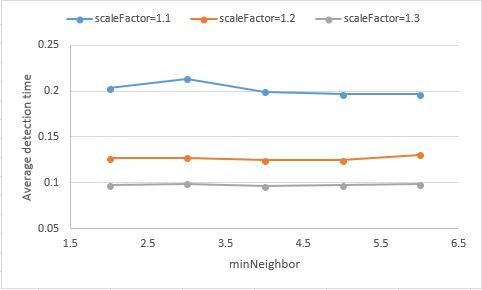
\includegraphics[height=4cm]{chap1/4.jpg}}
	\hspace{4em}
	\subcaptionbox{人脸大小占比图\label{fig:chap1:cfddb2}}
	{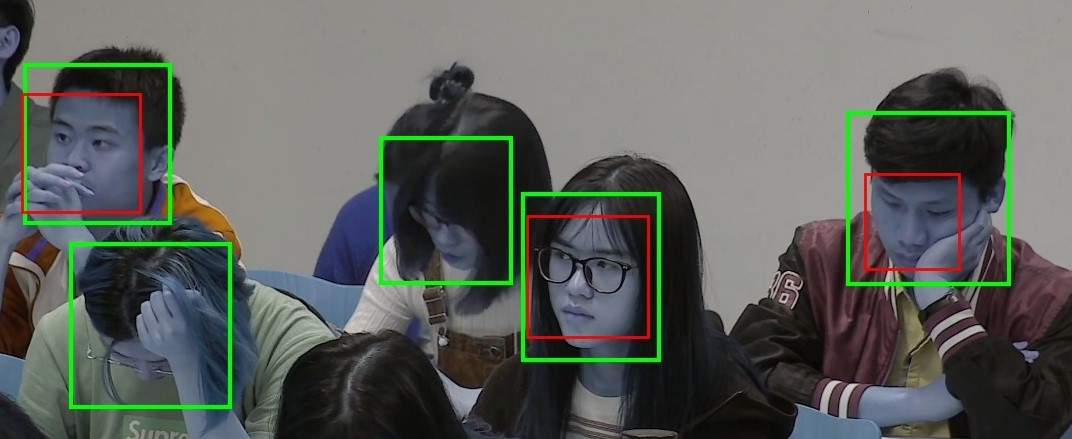
\includegraphics[height=4cm]{chap1/5.jpg}}
	\hspace{4em}
	\subcaptionbox{人脸遮挡占比图\label{fig:chap1:cfddb3}}
	{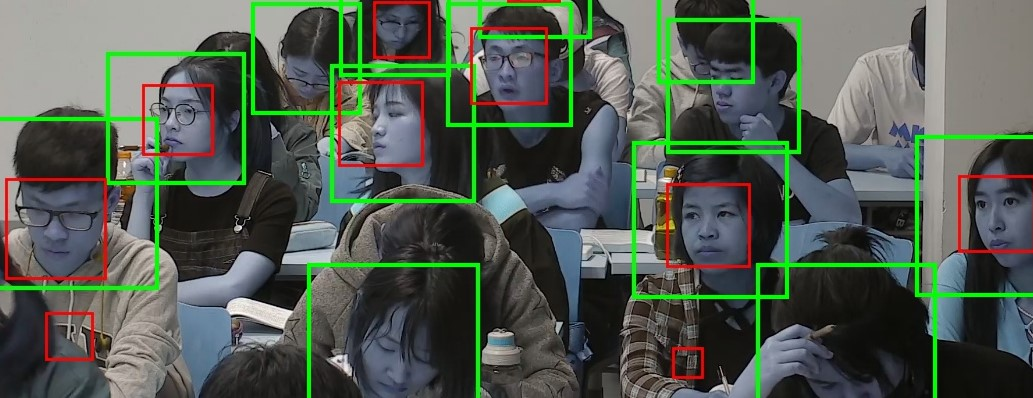
\includegraphics[height=4cm]{chap1/6.jpg}}
	\caption{CFDDB属性分析}
	\label{fig:cfddbeval}
\end{figure}

\section{CFDDB测试集的改进}

CFDDB由于采用了从视频流中截取连续帧的方法,使得有部分图片之间差异性较小。从而导致在测试检测算法时,如果在某张图片上效果不好,则在与之相邻的相同场景的图片上效果依然不好。这样会导致容易积累同样的错误从而使得CFDDB检测结果出现偏差。对于这种问题,可以通过使用更多的资源对数据库进行扩充来解决。如果数据量足够大,就可以稀释相似图片的积累错误,从而使得评价结果更加客观准确。

目前CFDDB采用通过剪裁截取到的图片计算类中心的方法建立人脸标准数据库。事实上这种方法只能粗略测得识别算法的准确性。更符合无感知检测场景的方法应当是由视频中出现人物的一张或多张证件照提取人脸特征向量,在对这些向量求类中心之后,得到人脸标准数据库中的人脸特征信息。目前受限于隐私保护,尚无法获得数据库中出现人脸的证件信息。这个问题有两种解决方法。第一种方法为招募志愿者,并提供完整的隐私保护政策,收集证件的照片信息。第二种方法为与受信任的机构合作,例如学校、医院,在学生或员工同意的情况下请机构提供证件的照片信息。

\section{CFDDB测试集的扩充}

限于人力和物力,CFDDB测试集目前数据量并不多。但是CFDDB在建立时就为可扩展性提供了广泛的支持。

首先,在标注人脸信息是使用了开源的工具labelImg\footnote{https://github.com/tzutalin/labelImg}与通用的XML模板。这使得即使对CFDDB测试集没有过多了解的人也可以非常容易的参与到CFDDB测试集的扩充中。其次,我们收集了多种教室类型的视频数据,并设计了开源的抽取程序,使得任何人都可以非常简单的按照与我们同样的标准抽取视频数据,在保证测试集数据一致性的基础上提升了效率。最后,我们提供了开源的XML处理程序和算法测试样例,方便更多的研究者参与和使用CFDDB数据集。

未来更多人有望能够参与到CFDDB的使用和扩充中,使得CFDDB可以成为特定场景的非受控无感知人脸检测和识别的先进测试集。如果数据量继续增加到数万张标记图片的规模,则可以将CFDDB中的数据按照某种合理的方式分为测试集和训练集,以方便对针对非受控无感知环境下人脸检测和识别算法的训练。

%# -*- coding: utf-8-unix -*-
%%==================================================
%% chapter02.tex for SJTU Master Thesis
%% based on CASthesis
%% modified by wei.jianwen@gmail.com
%% Encoding: UTF-8
%%==================================================

\chapter{{\LaTeX} 排版例子}
\label{chap:example}

\section{列表环境}
\label{sec:list}

\subsection{无序列表}
\label{sec:unorderlist}

以下是一个无序列表的例子,列表的每个条目单独分段。

\begin{itemize}
  \item 这是一个无序列表。
  \item 这是一个无序列表。
  \item 这是一个无序列表。
\end{itemize}

使用\verb+itemize*+环境可以创建行内无序列表。
\begin{itemize*}
  \item 这是一个无序列表。
  \item 这是一个无序列表。
  \item 这是一个无序列表。
\end{itemize*}
行内无序列表条目不单独分段,所有内容直接插入在原文的段落中。

\subsection{有序列表}
\label{sec:orderlist}

使用环境\verb+enumerate+和\verb+enumerate*+创建有序列表,
使用方法无序列表类似。

\begin{enumerate}
  \item 这是一个有序列表。
  \item 这是一个有序列表。
  \item 这是一个有序列表。
\end{enumerate}

使用\verb+enumerate*+环境可以创建行内有序列表。
\begin{enumerate*}
  \item 这是一个默认有序列表。
  \item 这是一个默认有序列表。
  \item 这是一个默认有序列表。
\end{enumerate*}
行内有序列表条目不单独分段,所有内容直接插入在原文的段落中。

\subsection{描述型列表}

使用环境\verb+description+可创建带有主题词的列表,条目语法是\verb+\item[主题] 内容+。
\begin{description}
    \item[主题一] 详细内容
    \item[主题二] 详细内容
    \item[主题三] 详细内容 \ldots
\end{description}

\subsection{自定义列表样式}

可以使用\verb+label+参数控制列表的样式,
详细可以参考WikiBooks\footnote{\url{https://en.wikibooks.org/wiki/LaTeX/List_Structures\#Customizing_lists}}。
比如一个自定义样式的行内有序列表
\begin{enumerate*}[label=\itshape\alph*)\upshape]
  \item 这是一个自定义样式有序列表。
  \item 这是一个自定义样式有序列表。
  \item 这是一个自定义样式有序列表。
\end{enumerate*}

\section{数学排版}
\label{sec:matheq}

\subsection{公式排版}
\label{sec:eqformat}

这里有举一个长公式排版的例子,来自\href{http://www.tex.ac.uk/tex-archive/info/math/voss/mathmode/Mathmode.pdf}{《Math mode》}:

\begin {multline}
  \frac {1}{2}\Delta (f_{ij}f^{ij})=
  2\left (\sum _{i<j}\chi _{ij}(\sigma _{i}-
    \sigma _{j}) ^{2}+ f^{ij}\nabla _{j}\nabla _{i}(\Delta f)+\right .\\
  \left .+\nabla _{k}f_{ij}\nabla ^{k}f^{ij}+
    f^{ij}f^{k}\left [2\nabla _{i}R_{jk}-
      \nabla _{k}R_{ij}\right ]\vphantom {\sum _{i<j}}\right )
\end{multline}

\subsection{SI单位}

使用\verb+siunitx+宏包可以方便地输入SI单位制单位,例如\verb+\SI{5}{\um}+可以得到\SI{5}{\um}。

\subsubsection{一个四级标题}
\label{sec:depth4}

这是全文唯一的一个四级标题。在这部分中将演示了mathtools宏包中可伸长符号(箭头、等号的例子)的例子。

\begin{displaymath}
    A \xleftarrow[n=0]{} B \xrightarrow[LongLongLongLong]{n>0} C 
\end{displaymath}

\begin{eqnarray}
  f(x) & \xleftrightarrow[]{A=B}  & B \\
  & \xleftharpoondown[below]{above} & B \nonumber \\
  & \xLeftrightarrow[below]{above} & B
\end{eqnarray}

又如:

\begin{align}
  \label{eq:none}
  & I(X_3;X_4)-I(X_3;X_4\mid{}X_1)-I(X_3;X_4\mid{}X_2) \nonumber \\
  = & [I(X_3;X_4)-I(X_3;X_4\mid{}X_1)]-I(X_3;X_4\mid{}\tilde{X}_2) \\
  = & I(X_1;X_3;X_4)-I(X_3;X_4\mid{}\tilde{X}_2)
\end{align}

\subsection{定理环境}

模板中定义了丰富的定理环境
algo(算法),thm(定理),lem(引理),prop(命题),cor(推论),defn(定义),conj(猜想),exmp(例),rem(注),case(情形),
bthm(断言定理),blem(断言引理),bprop(断言命题),bcor(断言推论)。
amsmath还提供了一个proof(证明)的环境。
这里举一个“定理”和“证明”的例子。
\begin{thm}[留数定理]
\label{thm:res}
  假设$U$是复平面上的一个单连通开子集,$a_1,\ldots,a_n$是复平面上有限个点,$f$是定义在$U\backslash \{a_1,\ldots,a_n\}$上的全纯函数,
  如果$\gamma$是一条把$a_1,\ldots,a_n$包围起来的可求长曲线,但不经过任何一个$a_k$,并且其起点与终点重合,那么:

  \begin{equation}
    \label{eq:res}
    \ointop_{\gamma}f(z)\,\mathrm{d}z = 2\uppi\mathbf{i}\sum^n_{k=1}\mathrm{I}(\gamma,a_k)\mathrm{Res}(f,a_k)
  \end{equation}

  如果$\gamma$是若尔当曲线,那么$\mathrm{I}(\gamma, a_k)=1$,因此:

  \begin{equation}
    \label{eq:resthm}
    \ointop_{\gamma}f(z)\,\mathrm{d}z = 2\uppi\mathbf{i}\sum^n_{k=1}\mathrm{Res}(f,a_k)
  \end{equation}

      % \oint_\gamma f(z)\, dz = 2\pi i \sum_{k=1}^n \mathrm{Res}(f, a_k ). 

  在这里,$\mathrm{Res}(f, a_k)$表示$f$在点$a_k$的留数,$\mathrm{I}(\gamma,a_k)$表示$\gamma$关于点$a_k$的卷绕数。
  卷绕数是一个整数,它描述了曲线$\gamma$绕过点$a_k$的次数。如果$\gamma$依逆时针方向绕着$a_k$移动,卷绕数就是一个正数,
  如果$\gamma$根本不绕过$a_k$,卷绕数就是零。

  定理\ref{thm:res}的证明。
  
  \begin{proof}
    首先,由……

    其次,……

    所以……
  \end{proof}
\end{thm}

上面的公式例子中,有一些细节希望大家注意。微分号d应该使用“直立体”也就是用mathrm包围起来。
并且,微分号和被积函数之间应该有一段小间隔,可以插入\verb+\,+得到。
斜体的$d$通常只作为一般变量。
i,j作为虚数单位时,也应该使用“直立体”为了明显,还加上了粗体,例如\verb+\mathbf{i}+。斜体$i,j$通常用作表示“序号”。
其他字母在表示常量时,也推荐使用“直立体”譬如,圆周率$\uppi$(需要upgreek宏包),自然对数的底$\mathrm{e}$。
不过,我个人觉得斜体的$e$和$\pi$很潇洒,在不至于引起混淆的情况下,我也用这两个字母的斜体表示对应的常量。


\section{向文档中插入图像}
\label{sec:insertimage}

\subsection{支持的图片格式}
\label{sec:imageformat}

\XeTeX 可以很方便地插入PDF、PNG、JPG格式的图片。

插入PNG/JPG的例子如\ref{fig:SRR}所示。
这两个水平并列放置的图共享一个“图标题”(table caption),没有各自的小标题。

\begin{figure}[!htp]
  \centering
  \includegraphics[width=4cm]{example/sjtulogo.png}
  \hspace{1cm}
  \includegraphics[width=4cm]{example/sjtulogo.jpg}
  \bicaption[这里将出现在插图索引中]
    {中文题图}
    {English caption}
  \label{fig:SRR}
\end{figure}

这里还有插入EPS图像和PDF图像的例子,如图\ref{fig:epspdf:a}和图\ref{fig:epspdf:b}。这里将EPS和PDF图片作为子图插入,每个子图有自己的小标题。子图标题使用subcaption宏包添加。

\begin{figure}[!htp]
  \centering
  \subcaptionbox{EPS 图像\label{fig:epspdf:a}}[3cm] %标题的长度,超过则会换行,如下一个小图。
    {\includegraphics[height=2.5cm]{example/sjtulogo.eps}}
  \hspace{4em}
  \subcaptionbox{PDF 图像,注意这个图略矮些。如果标题很长的话,它会自动换行\label{fig:epspdf:b}}
    {\includegraphics[height=2cm]{sjtulogo.pdf}}
  \bicaption{插入eps和pdf的例子(使用 subcaptionbox 方式)}{An EPS and PDF demo with subcaptionbox}
  \label{fig:pdfeps-subcaptionbox}
\end{figure}

\begin{figure}[!htp]
  \centering
  \begin{subfigure}{2.5cm}
    \centering
    \includegraphics[height=2.5cm]{example/sjtulogo.eps}
    \caption{EPS 图像}
  \end{subfigure}
  \hspace{4em}
  \begin{subfigure}{0.4\textwidth}
    \centering
    \includegraphics[height=2cm]{sjtulogo.pdf}
    \caption{PDF 图像,注意这个图略矮些。subfigure中同一行的子图在顶端对齐。}
  \end{subfigure}
  \bicaption{插入eps和pdf的例子(使用 subfigure 方式)}{An EPS and PDF demo with subfigure}
  \label{fig:pdfeps-subfigure}
\end{figure}

更多关于 \LaTeX 插图的例子可以参考\href{http://www.cs.duke.edu/junhu/Graphics3.pdf}{《\LaTeX 插图指南》}。

\subsection{长标题的换行}
\label{sec:longcaption}

图\ref{fig:longcaptionbad}和图\ref{fig:longcaptiongood}都有比较长图标题,通过对比发现,图\ref{fig:longcaptiongood}的换行效果更好一些。
其中使用了minipage环境来限制整个浮动体的宽度。

\begin{figure}[!htp]
  \centering
  \includegraphics[width=4cm]{sjtubadge.pdf}
  \bicaption[这里将出现在插图索引]
    {上海交通大学是我国历史最悠久的高等学府之一,是教育部直属、教育部与上海市共建的全国重点大学.}
    {Where there is a will, there is a way.}
 \label{fig:longcaptionbad}
\end{figure}

\begin{figure}[!htbp]
  
  \begin{minipage}[b]{0.6\textwidth}
    \centering
    \includegraphics[width=4cm]{sjtubadge.pdf}
    \bicaption[出现在插图索引中]
      {上海交通大学是我国历史最悠久的高等学府之一,是教育部直属、教育部与上海市共建的全国重点大学.}
      {Where there is a will, there is a way.}
    \label{fig:longcaptiongood}
  \end{minipage}     
\end{figure}

\subsection{绘制流程图}

图\ref{fig:flow_chart}是一张流程图示意。使用tikz环境,搭配四种预定义节点(\verb+startstop+、\verb+process+、\verb+decision+和\verb+io+),可以容易地绘制出流程图。
\begin{figure}[!htp]
    \centering
    \resizebox{6cm}{!}{\input{figure/example/flow_chart.tex}}
    \bicaption{绘制流程图效果}{Flow chart}
    \label{fig:flow_chart}
\end{figure}
  
\clearpage

\section{表格}
\label{sec:tab}

这一节给出的是一些表格的例子,如表\ref{tab:firstone}所示。

\begin{table}[!hpb]
  \centering
  \bicaption[指向一个表格的表目录索引]
    {一个颇为标准的三线表格\footnotemark[1]}
    {A Table}
  \label{tab:firstone}
  \begin{tabular}{@{}llr@{}} \toprule
    \multicolumn{2}{c}{Item} \\ \cmidrule(r){1-2}
    Animal & Description & Price (\$)\\ \midrule
    Gnat & per gram & 13.65 \\
    & each & 0.01 \\
    Gnu & stuffed & 92.50 \\
    Emu & stuffed & 33.33 \\
    Armadillo & frozen & 8.99 \\ \bottomrule
  \end{tabular}
\end{table}
\footnotetext[1]{这个例子来自\href{http://www.ctan.org/tex-archive/macros/latex/contrib/booktabs/booktabs.pdf}{《Publication quality tables in LATEX》}(booktabs宏包的文档)。这也是一个在表格中使用脚注的例子,请留意与threeparttable实现的效果有何不同。}

下面一个是一个更复杂的表格,用threeparttable实现带有脚注的表格,如表\ref{tab:footnote}。

\begin{table}[!htpb]
  \bicaption[出现在表目录的标题]
    {一个带有脚注的表格的例子}
    {A Table with footnotes}
  \label{tab:footnote}
  \centering
  \begin{threeparttable}[b]
     \begin{tabular}{ccd{4}cccc}
      \toprule
      \multirow{2}{6mm}{total}&\multicolumn{2}{c}{20\tnote{1}} & \multicolumn{2}{c}{40} &  \multicolumn{2}{c}{60}\\
      \cmidrule(lr){2-3}\cmidrule(lr){4-5}\cmidrule(lr){6-7}
      &www & \multicolumn{1}{c}{k} & www & k & www & k \\ % 使用说明符 d 的列会自动进入数学模式,使用 \multicolumn 对文字表头做特殊处理
      \midrule
      &$\underset{(2.12)}{4.22}$ & 120.0140\tnote{2} & 333.15 & 0.0411 & 444.99 & 0.1387 \\
      &168.6123 & 10.86 & 255.37 & 0.0353 & 376.14 & 0.1058 \\
      &6.761    & 0.007 & 235.37 & 0.0267 & 348.66 & 0.1010 \\
      \bottomrule
    \end{tabular}
    \begin{tablenotes}
    \item [1] the first note.% or \item [a]
    \item [2] the second note.% or \item [b]
    \end{tablenotes}
  \end{threeparttable}
\end{table}

\section{参考文献管理}

 \LaTeX 具有将参考文献内容和表现形式分开管理的能力,涉及三个要素:参考文献数据库、参考文献引用格式、在正文中引用参考文献。
这样的流程需要多次编译:

\begin{enumerate}[noitemsep,topsep=0pt,parsep=0pt,partopsep=0pt]
	\item 用户将论文中需要引用的参考文献条目,录入纯文本数据库文件(bib文件)。
	\item 调用xelatex对论文模板做第一次编译,扫描文中引用的参考文献,生成参考文献入口文件(aux)文件。
	\item 调用bibtex,以参考文献格式和入口文件为输入,生成格式化以后的参考文献条目文件(bib)。
	\item 再次调用xelatex编译模板,将格式化以后的参考文献条目插入正文。
\end{enumerate}

参考文献数据库(thesis.bib)的条目,可以从Google Scholar搜索引擎\footnote{\url{https://scholar.google.com}}、CiteSeerX搜索引擎\footnote{\url{http://citeseerx.ist.psu.edu}}中查找,文献管理软件Papers\footnote{\url{http://papersapp.com}}、Mendeley\footnote{\url{http://www.mendeley.com}}、JabRef\footnote{\url{http://jabref.sourceforge.net}}也能够输出条目信息。

下面是在Google Scholar上搜索到的一条文献信息,格式是纯文本:

\begin{lstlisting}[caption={从Google Scholar找到的参考文献条目}, label=googlescholar, escapeinside="", numbers=none]
    @phdthesis{"白2008信用风险传染模型和信用衍生品的定价",
      title={"信用风险传染模型和信用衍生品的定价"},
      author={"白云芬"},
      year={2008},
      school={"上海交通大学"}
    } 
\end{lstlisting}

推荐修改后在bib文件中的内容为:

\begin{lstlisting}[caption={修改后的参考文献条目}, label=itemok, escapeinside="", numbers=none]
  @phdthesis{bai2008,
    title={"信用风险传染模型和信用衍生品的定价"},
    author={"白云芬"},
    date={2008},
    address={"上海"},
    school={"上海交通大学"}
  } 
\end{lstlisting}

按照教务处的要求,参考文献外观应符合国标GBT7714的要求\footnote{\url{http://www.cces.net.cn/guild/sites/tmxb/Files/19798_2.pdf}}。
在模板中,表现形式的控制逻辑通过biblatex-gb7714-2015包实现\footnote{\url{https://www.ctan.org/pkg/biblatex-gb7714-2015}},基于{Bib\LaTeX}管理文献。在目前的多数TeX发行版中,可能都没有默认包含biblatex-gb7714-2015,需要手动安装。

正文中引用参考文献时,用\verb+\cite{key1,key2,key3...}+可以产生“上标引用的参考文献”,
如\cite{Meta_CN,chen2007act,DPMG}。
使用\verb+\parencite{key1,key2,key3...}+则可以产生水平引用的参考文献,例如\parencite{JohnD,zhubajie,IEEE-1363}。
请看下面的例子,将会穿插使用水平的和上标的参考文献:关于书的\parencite{Meta_CN,JohnD,IEEE-1363},关于期刊的\cite{chen2007act,chen2007ewi},
会议论文\parencite{DPMG,kocher99,cnproceed},
硕士学位论文\parencite{zhubajie,metamori2004},博士学位论文\cite{shaheshang,FistSystem01,bai2008},标准文件\parencite{IEEE-1363},技术报告\cite{NPB2},电子文献\parencite{xiaoyu2001, CHRISTINE1998},用户手册\parencite{RManual}。

总结一些注意事项:
\begin{itemize}
\item 参考文献只有在正文中被引用了,才会在最后的参考文献列表中出现;
\item 参考文献“数据库文件”bib是纯文本文件,请使用UTF-8编码,不要使用GBK编码;
\item 参考文献条目中默认通过date域输入时间。兼容使用year域时会产生编译warning,可忽略。
\end{itemize}

\section{用listings插入源代码}

原先ctexbook文档类和listings宏包配合使用时,代码在换页时会出现莫名其妙的错误,后来经高人指点,顺利解决了。
感兴趣的话,可以看看\href{http://bbs.ctex.org/viewthread.php?tid=53451}{这里}。
这里给使用listings宏包插入源代码的例子,这里是一段C代码。
另外,listings宏包真可谓博大精深,可以实现各种复杂、漂亮的效果,想要进一步学习的同学,可以参考
\href{http://mirror.ctan.org/macros/latex/contrib/listings/listings.pdf}{listings宏包手册}。

\begin{lstlisting}[language={C}, caption={一段C源代码}]
#include <stdio.h>
#include <unistd.h>
#include <sys/types.h>
#include <sys/wait.h>

int main() {
  pid_t pid;

  switch ((pid = fork())) {
  case -1:
    printf("fork failed\n");
    break;
  case 0:
    /* child calls exec */
    execl("/bin/ls", "ls", "-l", (char*)0);
    printf("execl failed\n");
    break;
  default:
    /* parent uses wait to suspend execution until child finishes */
    wait((int*)0);
    printf("is completed\n");
    break;
  }

  return 0;
}
\end{lstlisting}

\section{用algorithm和algorithmicx宏包插入算法描述}

algorithmicx 比 algorithmic 增加了一些命令。
示例如算法\ref{algo:sum_100}和算法\ref{algo:merge_sort},
后者的代码来自\href{http://hustsxh.is-programmer.com/posts/38801.html}{xhSong的博客}。
algorithmicx的详细使用方法见\href{http://mirror.hust.edu.cn/CTAN/macros/latex/contrib/algorithmicx/algorithmicx.pdf}{官方README}。
使用算法宏包时,算法出现的位置很多时候不按照tex文件里的书写顺序, 
需要强制定位时可以使用\verb+\begin{algorithm}[H]+
\footnote{http://tex.stackexchange.com/questions/165021/fixing-the-location-of-the-appearance-in-algorithmicx-environment}

这是写在算法\ref{algo:sum_100}前面的一段话,在生成的文件里它会出现在算法\ref{algo:sum_100}前面。

\begin{algorithm}
% \begin{algorithm}[H] % 强制定位
\caption{求100以内的整数和}
\label{algo:sum_100}
\begin{algorithmic}[1] %每行显示行号
\Ensure 100以内的整数和 % 输出
\State $sum \gets 0$
\For{$i = 0 \to 100$}
    \State $sum \gets sum + i$
  \EndFor
\end{algorithmic}
\end{algorithm}

这是写在两个算法中间的一段话,当算法\ref{algo:sum_100}不使用\verb+\begin{algorithm}[H]+时它也会出现在算法\ref{algo:sum_100}前面。

对于很长的算法,单一的算法块\verb+\begin{algorithm}...\end{algorithm}+是不能自动跨页的
\footnote{http://tex.stackexchange.com/questions/70733/latex-algorithm-not-display-under-correct-section},
会出现的情况有:

\begin{itemize}
  \item 该页放不下当前的算法,留下大片空白,算法在下一页显示
  \item 单一页面放不下当前的算法,显示时超过页码的位置直到超出整个页面范围
\end{itemize}

解决方法有:

\begin{itemize}
  \item (推荐)使用\verb+algstore{algname}+和\verb+algrestore{algname}+来讲算法分为两个部分\footnote{http://tex.stackexchange.com/questions/29816/algorithm-over-2-pages},如算法\ref{algo:merge_sort}。
  \item 人工拆分算法为多个小的部分。
\end{itemize}

\begin{algorithm}
% \begin{algorithm}[H] % 强制定位
\caption{用归并排序求逆序数}
\label{algo:merge_sort}
\begin{algorithmic}[1] %每行显示行号
\Require $Array$数组,$n$数组大小 % 输入
\Ensure 逆序数 % 输出
\Function {MergerSort}{$Array, left, right$}
  \State $result \gets 0$
  \If {$left < right$}
    \State $middle \gets (left + right) / 2$
    \State $result \gets result +$ \Call{MergerSort}{$Array, left, middle$}
    \State $result \gets result +$ \Call{MergerSort}{$Array, middle, right$}
    \State $result \gets result +$ \Call{Merger}{$Array,left,middle,right$}
  \EndIf
  \State \Return{$result$}
\EndFunction
\State %空一行
\Function{Merger}{$Array, left, middle, right$}
  \State $i\gets left$
  \State $j\gets middle$
  \State $k\gets 0$
  \State $result \gets 0$
  \While{$i<middle$ \textbf{and} $j<right$}
    \If{$Array[i]<Array[j]$}
      \State $B[k++]\gets Array[i++]$
    \Else
      \State $B[k++] \gets Array[j++]$
      \State $result \gets result + (middle - i)$
    \EndIf
  \EndWhile
  \algstore{MergeSort}
\end{algorithmic}
\end{algorithm}

\begin{algorithm}
\begin{algorithmic}[1]
  \algrestore{MergeSort}
  \While{$i<middle$}
    \State $B[k++] \gets Array[i++]$
  \EndWhile
  \While{$j<right$}
    \State $B[k++] \gets Array[j++]$
  \EndWhile
  \For{$i = 0 \to k-1$}
    \State $Array[left + i] \gets B[i]$
  \EndFor
  \State \Return{$result$}
\EndFunction
\end{algorithmic}
\end{algorithm}

这是写在算法\ref{algo:merge_sort}后面的一段话,
但是当算法\ref{algo:merge_sort}不使用\verb+\begin{algorithm}[H]+时它会出现在算法\ref{algo:merge_sort}
甚至算法\ref{algo:sum_100}前面。

对于算法的索引要注意\verb+\caption+和\verb+\label+的位置, 
必须是先\verb+\caption+再\verb+\label+\footnote{http://tex.stackexchange.com/questions/65993/algorithm-numbering},
否则会出现\verb+\ref{algo:sum_100}+生成的编号跟对应算法上显示不一致的问题。

根据Werner的回答\footnote{http://tex.stackexchange.com/questions/53357/switch-cases-in-algorithmic}
增加了\verb+Switch+和\verb+Case+的支持,见算法\ref{algo:switch_example}。

\begin{algorithm}
\caption{Switch示例}
\label{algo:switch_example}
\begin{algorithmic}[1]
  \Switch{$s$}
    \Case{$a$}
      \Assert{0}
    \EndCase
    \Case{$b$}
      \Assert{1}
    \EndCase
    \Default
      \Assert{2}
    \EndDefault
  \EndSwitch
\end{algorithmic}
\end{algorithm}

\include{tex/faq}
%# -*- coding: utf-8-unix -*-
%%==================================================
%% conclusion.tex for SJTUThesis
%% Encoding: UTF-8
%%==================================================

\begin{summary}

本文针对无感知环境下的大规模人脸数据的模糊搜索,从五个方面开展研究:

第一,建立无感知人脸检测的数据集CFDDB。并在CFDDB上定义召回率$recall$、误判率$errorrate$与检测参数$\alpha$等测试基准。之后进行人脸数据属性分析,探讨数据集的改进方法,制定数据集的扩充流程。

第二,根据CFDDB测试集的基准定义,完成四种不同的人脸检测算法的封装测试与参数调优。根据测试结果,选择SSH检测器\cite{najibi2017ssh}作为系统人脸检测模块的核心。

第三,利用CFDDB中的数据,对InsightFace\cite{deng2018arcface}进行测试,并将其封装为系统的人脸识别模块。

第四,针对小规模数据匹配,提出线性搜索和多类支持向量机两种方案。针对大规模数据匹配,研究基于局部敏感哈希与基于有向图的两种近似搜索算法,并提出优化思路。

第五,高效、稳定、可扩展的系统架构设计。

综合以上五方面的研究成果,最终在GPU服务器上实现了无感知人脸识别系统。

\end{summary}


\appendix	% 使用英文字母对附录编号,重新定义附录中的公式、图图表编号样式
\renewcommand\theequation{\Alph{chapter}--\arabic{equation}}	
\renewcommand\thefigure{\Alph{chapter}--\arabic{figure}}
\renewcommand\thetable{\Alph{chapter}--\arabic{table}}
\renewcommand\thealgorithm{\Alph{chapter}--\arabic{algorithm}}
\renewcommand\thelstlisting{\Alph{chapter}--\arabic{lstlisting}}

%% 附录内容,本科学位论文可以用翻译的文献替代。
\include{tex/app_setup}
\include{tex/app_eq}
\include{tex/app_cjk}
\include{tex/app_log}

\backmatter	% 文后无编号部分 

%% 参考资料
\printbibliography[heading=bibintoc]

%% 致谢、发表论文、申请专利、参与项目、简历
%% 用于盲审的论文需隐去致谢、发表论文、申请专利、参与的项目
\makeatletter

%%
% "研究生学位论文送盲审印刷格式的统一要求"
% http://www.gs.sjtu.edu.cn/inform/3/2015/20151120_123928_738.htm

% 盲审删去删去致谢页
\ifsjtu@review\relax\else
  %# -*- coding: utf-8-unix -*-
\begin{thanks}

  感谢沈耀老师提供实验场所和悉心指导!

  感谢郁东风同学提供训练好的人脸识别模型!

  感谢沈国栋学长在实验环境搭建和服务器搭建给予我的帮助!
  
  感谢龚桂学长在小脸检测和嵌入式设备运行方面给予我的帮助!
  
  感谢孙泽堃、郭远帆、丁志勇和罗翔中同学志愿参与CFDDB测试集的标注!
  
  感谢其他所有帮助我的同学和老师!

\end{thanks}
 	  %% 致谢
\fi

\ifsjtu@bachelor
  % 学士学位论文要求在最后有一个英文大摘要,单独编页码
  \pagestyle{biglast}
  %# -*- coding: utf-8-unix -*-
\begin{bigabstract}

ENGLISH

\end{bigabstract}
\else
  % 盲审论文中,发表学术论文及参与科研情况等仅以第几作者注明即可,不要出现作者或他人姓名
  \ifsjtu@review\relax
    \include{tex/pubreview}
    \include{tex/projectsreview}  
  \else
    \include{tex/pub}	      %% 发表论文
    \include{tex/projects}  %% 参与的项目
  \fi
\fi

% \include{tex/patents}	  %% 申请专利
% \include{tex/resume}	  %% 个人简历

\makeatother

\end{document}
